% OWD 2024
%
\documentclass{beamer}
\usepackage{caption}

\usetheme{Berlin}
\numberwithin{figure}{section}
\beamerdefaultoverlayspecification{< +->}
\setbeamertemplate{headline}{}
\setbeamertemplate{page number in head/foot}[framenumber]

\newcommand\gamename{\emph{Heslington Hustle}}
\newcommand\groupname{Byte Musketeers}

\title{\gamename\ Product Demonstration}
\author[\groupname]{%
    \texorpdfstring{
\includegraphics[width=0.3\linewidth]{../logo}}{\groupname}}

\institute{Department of Computer Science, University of York}
\date{Semester 2, 2024}

\begin{document}
\frame{\titlepage}
\begin{frame}
    \frametitle{Game Demonstration}
    \begin{figure}
        \setlength\fboxsep{0pt}
        \begin{tabular}{@{\hspace{1ex}}c@{\hspace{1ex}}c@{\hspace{1ex}}c}
            \fbox{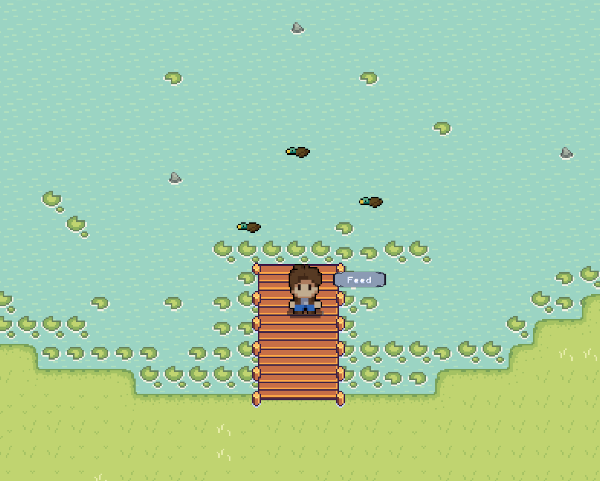
\includegraphics[width=.3\linewidth]{assets/ducks}} &
            \fbox{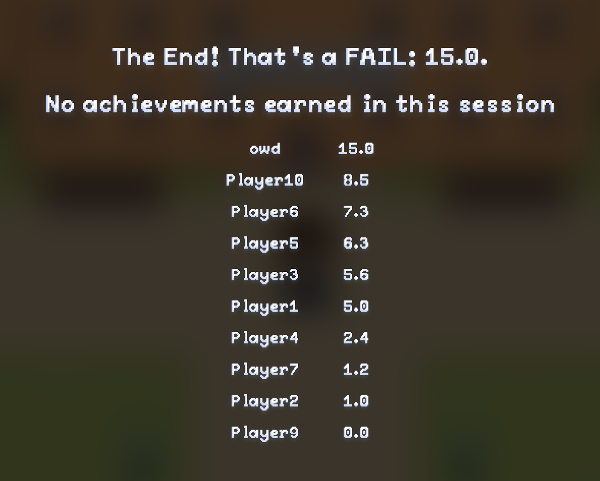
\includegraphics[width=.3\linewidth]{assets/leaderboard}} &
            \fbox{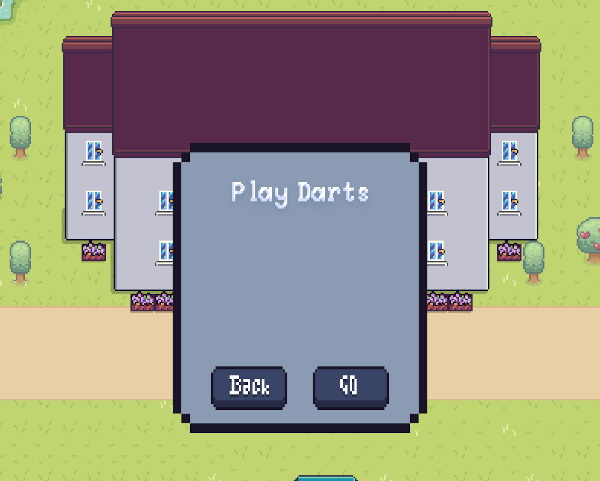
\includegraphics[width=.3\linewidth]{assets/darts}}
        \end{tabular}
        \caption*{\gamename\ Game Demonstration}
    \end{figure}
\end{frame}
\begin{frame}
    \frametitle{Technical Overview}
    \begin{itemize}
        \item \textbf{Comprehensive Testing.} A conjunction of automated and
            manual testing by members of the development team and external
            testers. \emph{Product correctness} is guaranteed and verifiable.
        \item \textbf{Modular and Extensible.} Minimal programming is required
            to add new areas; on-boarding future development teams is trivial.
        \item \textbf{Numerous Vectors for Monetisation.} Modularity of the
            code-base encourages and actively supports the development of
            substantial extensions, such as additional areas in the form of
            downloadable content (DLC).
    \end{itemize}
\end{frame}
\begin{frame}
    \frametitle{Market Potential}
    \begin{itemize}
        \item \textbf{Attractive for Third-Party Commercialisation.} Easily
            swappable assets enable quick adoption of brand deals with third
            parties, such as universities, students' unions, and local public
            transport providers.
        \item \textbf{Continual Revenue Streams.} Character skins; in-game
            currencies; level bonuses: all likely mechanisms of creating stable
            cash-flow streams through \emph{micro-transactions}.
        \item \textbf{Strong Knowledge of the Player.} Substantial market
            research analysis was performed on a sample of the target audience:
            16-to-25-year-olds enrolling at an HE institution.
        \item \textbf{Inherently Cross-Platform.} Java and LibGDX provide proven
            stability across Windows, Mac, and Linux. The framework for mobile
            support is in place.
    \end{itemize}
\end{frame}
\begin{frame}
    \frametitle{User Evaluation Feedback}
    \centering
    \renewcommand\arraystretch{2}
    \begin{tabular}{p{.44\linewidth}@{\hspace{3ex}}p{.44\linewidth}}
        \emph{What did the customers say?} & \emph{How did we respond?} \\
        \hline
        Attempted to enter inactive buildings & Added interactable activities to
        all buildings\pause \\
        Some unexpected parts of the map were accessible & Made the map more
        navigable with visual boundaries\pause \\
        The achievements system was unintuitive & Improved the end-screen to
        provide a comprehensive summary of the game session\pause
    \end{tabular}
    \vfill\textbf{We know your customer!}
\end{frame}
\begin{frame}
    \frametitle{Licensing}
    \begin{center}
        
\includegraphics[width=.5\linewidth]{assets/cc-logo}
    \end{center}
    \begin{itemize}
        \item All in-game assets are suitably licensed under permissive
            conditions for commercial use.
        \item Assets used are constituents of \emph{asset packs}: a consistent
            art-style can be maintained for any extensions.
        \item Any IP created by the \emph{\groupname} is under an exclusive
            licence to be used by the proprietors of \gamename.
    \end{itemize}
\end{frame}
\begin{frame}
    \frametitle{Questions}
    \begin{figure}
        
\includegraphics[width=0.3\linewidth]{../logo}
        \vfill\caption*{\Large Any Questions?}
    \end{figure}
\end{frame}
\end{document}

